\newcommand{\numopensource}{5\xspace}
\subsection{Evaluation}
\label{shreds:sec:eval}

Our evaluation sought to answer the following questions: 
\begin{itemize}
%\item How easy or difficult for developers to adopt shreds in their code?
\item How compatible and useful are shreds to real-world programs?
\item How do shreds affect the application's and system's performance?
\item How shreds help mitigate in-process memory abuse?
\end{itemize}

\point{Choice of Applications}
We selected 5 popular open source applications to evaluate our prototype system.  The applications are shown in Table~\ref{tbl:apps}, ranging from the small HTTP server, lighttpd, to the complex cryptography library, OpenSSL. 
The applications were chosen because each of them has at least one piece of sensitive data that is subject to in-process abuse, and therefore, warrants shred's protection. Moreover, the applications represent a good variety of software of different functionalities and codebase sizes. 


\begin{table*}[]
\normalsize
\centering
\caption{5 open source softwares used in evaluation}
\label{tbl:apps}
%\resizebox{\columnwidth}{!}
{%
\begin{tabular}{|c|c|c|c|c|}
\hline
         & Executable Size(byte)                                                 & Category               & Protected Data Type         & Program Size(KLOC) \\ \hline
curl     & 227071 curl                                                           & http client   & password               & 177                \\ \hline
minizip  & \begin{tabular}[c]{@{}c@{}}80572 miniunz\\ 97749 minizip\end{tabular} & file compression tool  & password               & 7                  \\ \hline
openssh  & 2207588 ssh                                                           & remote login tool      & credential             & 130                \\ \hline
%openvpn  & 2351540 openvpn                                                       & network tool           & sensitive object & 173                \\ \hline
openssl  & 3093920 libcrypto.so                                                  & crypto library         & crypto key             & 526                \\ \hline
lighttpd & 85135 mod\_auth.so                                                    & web server & credential               & 56                 \\ \hline
%tor      & 5595518 tor                                                           & network proxy tool     & crypto key             & 236                \\ \hline
\end{tabular}%
}
\end{table*}

%    
%\point{Adoption Tests}
%To measure the efforts required to adopt shreds in reality, 
%we hired several CS graduate students to incorporate shreds into the 5 selected applications. They were first given a short tutorial on how to use shreds and s-pools, and then asked to adopt shreds into the application source code. The adoption in these tests did not intend to protect all kinds of sensitive data in the applications, which is unrealistic given that the student participants in the tests are not the original developers of the applications and are unlikely to identify all types of sensitive data. Instead, we asked the participants to protect only one specific type of sensitive data in each application (as shown in the Protected Data Type column in Table~\ref{tbl:apps}. This measurable and realistic task for the participants allowed us to examine how easy or difficult to use shreds correctly and effectively in practice. 
%
%After the tests finished, we manually confirmed the correctness and completeness of the code changes. The modified applications compile and run without any issue. 
%As shown in Table~\ref{fig:adopteffort}, on average, the participants spent an hour on lighttpd and 15 min on minizip, representing the longest and shortest adoption time measured in the tests. These numbers show that shreds are intuitive even to first-time users. Given that the participants spent most of the time understanding the codebase, we expect that the  time needed for adopting shreds will be even shorter when the original application developers perform the tasks. The number of shreds created and the number of SLoC changes do not exhibit direct correlation with the adoption time. The code changes are very small compared with the size of the applications, which indicates that no major design changes are required to apply shreds to existing applications. 
%
%
%\begin{table}[htbp]
%\begin{center}
%\caption{Code changed and time spent in adoption tests}
%\label{fig:adopteffort}
%\includegraphics[scale=0.7]{fig/adoptionEffort}
%\end{center}
%\end{table}

\point{Compilation Tests}
To test the performance and compatibility of our offline analysis and compilation methods, we instrumented S-compiler in order to measure the overhead and log potential errors, if any, while building  the \numopensource software packages that use shreds. 
Figure~\ref{fig:compile} shows the time and space overhead introduced by S-compiler, relative to the performance of a vanilla LLVM Clang compiling the unchanged applications. On average, S-compiler delays the building process by 24.58\% and results in a 7.37\% increase in executable sizes. The seemingly significant delays in compilation are in fact on par with static analysis and program instrumentation tools of similar scale. They are generally tolerable because compilations take place offline in background and are usually not considered to be time-critical. The executable file size increases are mainly resulted from the in-shred instrumentation and are below 2\% except for the outliers. 
%
%Compared with the vanilla LLVM Clang compiler, S-compiler increases the end-to-end compilation time by 9.59\% on average across all the tested software. This level of compilation delay is expected and generally tolerable because compilations take place offline often in background and are usually not considered to be time-critical. 
%We also counted the number of IR instructions that were inserted into each of the software for instrumentation purposes. The resulting binaries on average are 3.04\% larger in size than their originals. 
We encountered no error when building these applications using S-compiler. The built applications run without issues during the course of the tests. 
%Table~\ref{tbl:compile} shows the detailed results, which indicate S-compiler can analyze, instrument, and build very complex software without issues. 



\begin{figure*}[tbp]
	\centering
	\begin{minipage}[b]{0.4\textwidth}
		\centering	
			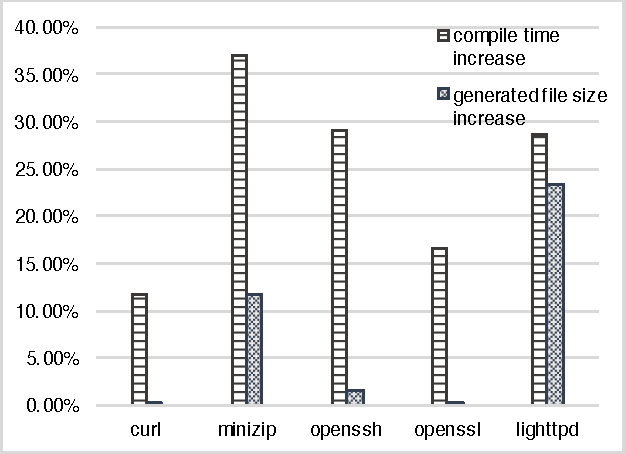
\includegraphics[scale=0.85]{shreds/figures/compile_overhead}
			\caption{The time and space overhead incurred by S-compiler during the offline compilation and instrumentation phase}
			\label{fig:compile}
	\end{minipage}
 \hfill
	\begin{minipage}[b]{0.4\textwidth}
		\centering	
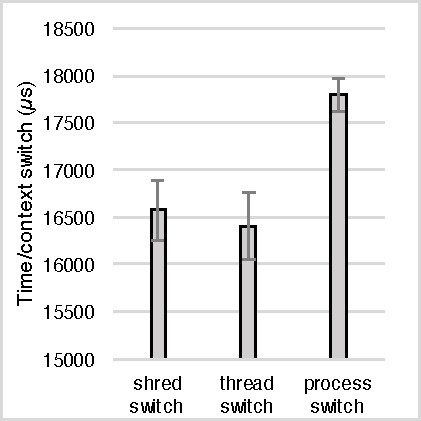
\includegraphics[scale=0.8]{shreds/figures/ctx_switch}
\caption{The time needed for a context switch when: (1) a shred-active thread is switched off, (2) a regular thread is switched off but no process or address space change,  and (3) a regular thread is switched off and a thread from a different process is scheduled on.}
\label{fig:ctxswtich}
	\end{minipage}
\end{figure*}


%\begin{figure}[htbp]
%\begin{center}
%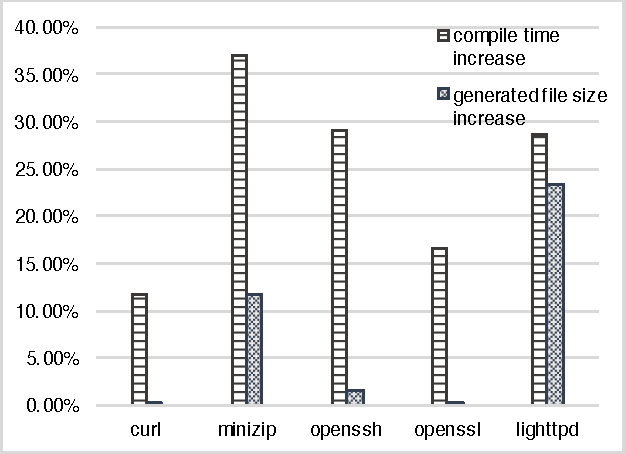
\includegraphics[scale=0.85]{shreds/figures/compile_overhead}
%\caption{The time and space overhead incurred by S-compiler during the offline compilation and instrumentation phase}
%\label{fig:compile}
%\end{center}
%\end{figure}
    
\point{Performance Tests}
%micro bench markings
This group of tests examines the runtime performance of shreds and s-pools. We performed both micro-benchmarkings and end-to-end tests, which respectively reveal the performance cost associated with shreds' critical operations and the overhead exhibited in the \numopensource applications retrofitted with shreds. 

In the micro-benchmarking tests, we developed unit test programs that force shreds to go through the critical operations and state changes, including shred entry, exit, and context switch. We measured the duration of these operations and state changes, and then compared them with the durations of the equivalent or related operations without shreds. Figure~\ref{fig:ctxswtich} shows the absolute time needed for a context switch that preempts a shred-active thread, a regular thread, and a regular process, respectively.   It is obvious that, switching shred-active threads is marginally more expensive than switching  regular threads ((about $100\mu s$ slower); switching shred-active threads is much faster than a process context switch. 
This is because when a shred is preempted, S-driver does not need to make any change to page tables or TLB. Instead, it only performs a single DACR reset operation, which is very lightweight. 

We also compared the time needed for completing the shred API calls (invoking {\tt ioctl} internally) with several reference system calls, as shown in Figure~\ref{fig:primitive}. The {\tt getpid}, one of the fastest system calls,  serves as a baseline for comparison. The {\tt shred\_enter} API is compared with the {\tt clone} system call (without address space change), and is slightly faster, which means creating a shred takes less time than creating a thread. The s-pool allocation API is mildly slower than {\tt mmap} due to the additional domain configurations.  But the overhead is low enough to easily blend in the typical  program performance fluctuations. 

Furthermore, we measured the performance improvement enabled by the lazy domain adjustment optimization. We applied shreds to five SPEC CINT2006 benchmark programs written in C (Figure~\ref{fig:sysoverhead}), where a number of shreds were created to perform intensive access to s-pools. We note that this test is designed only for the performance evaluation purpose while recognizing that these benchmark programs do not need shreds' protection. The result shows that in all but one case the optimization brings the overhead under 1\% whereas the non-optimized implementation of shreds incurs an average overhead of 2.5\%. 

Those micro-benchmark tests together indicate that the shred primitives are lightweight and the performance impact that shred state changes and s-pool operations may pose to the application or the system is very mild. 

%\begin{figure}[htbp]
%\begin{center}
%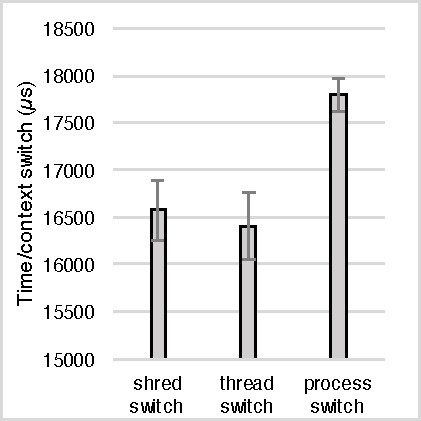
\includegraphics[scale=0.8]{shreds/figures/ctx_switch}
%\caption{The time needed for a context switch when: (1) a shred-active thread is switched off, (2) a regular thread is switched off but no process or address space change,  and (3) a regular thread is switched off and a thread from a different process is scheduled on.}
%\label{fig:ctxswtich}
%\end{center}
%\end{figure}

\begin{figure*}[htbp]
	\centering
	\begin{minipage}[b]{0.4\textwidth}
		\centering	
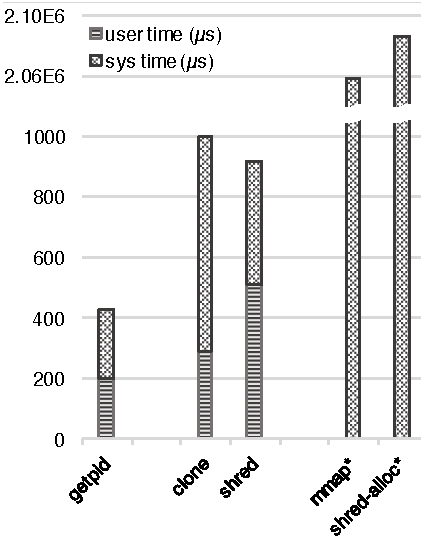
\includegraphics[scale=0.85]{shreds/figures/prim_compare}
\caption{Invocation time of shred APIs and reference system calls (the right-most two bars are on log scale). It shows that shred entry is faster than thread creation, and s-pool allocation is slightly slower than basic memory mapping.}
\label{fig:primitive}
	\end{minipage}
 \hfill
	\begin{minipage}[b]{0.4\textwidth}
		\centering	
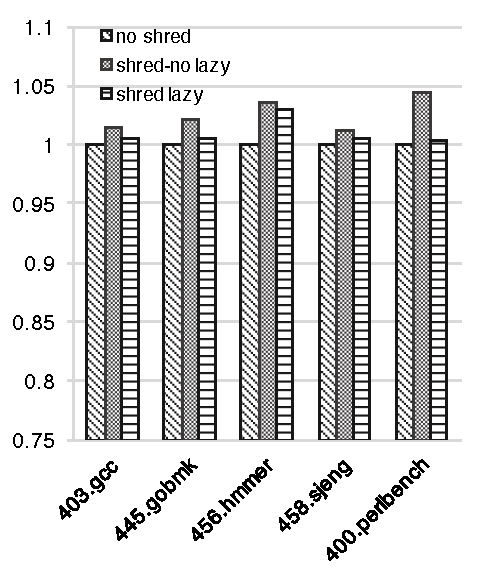
\includegraphics[scale=0.75]{shreds/figures/system_overhead}
\caption{Five SPEC2000 benchmark programs tested when: (1) no shred is used, (2) shreds are used but without the lazy domain adjustment turned on in S-driver, and (3) shreds are used with the lazy domain adjustment. }
\label{fig:sysoverhead}
	\end{minipage}
\end{figure*}

%\begin{figure}[htbp]
%\begin{center}
%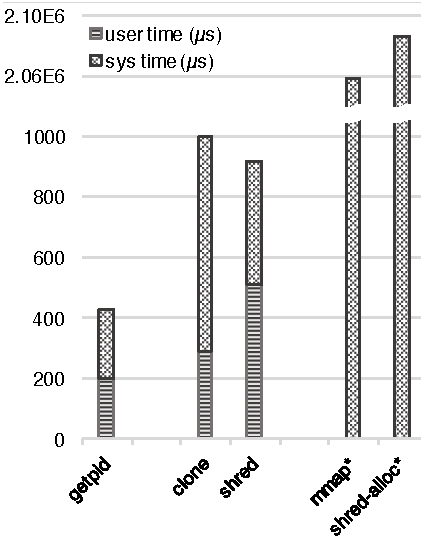
\includegraphics[scale=0.85]{shreds/figures/prim_compare}
%\caption{Invocation time of shred APIs and reference system calls (the right-most two bars are on log scale). It shows that shred entry is faster than thread creation, and s-pool allocation is slightly slower than basic memory mapping.}
%\label{fig:primitive}
%\end{center}
%\end{figure}
%
%
%\begin{figure}[htbp]
%\begin{center}
%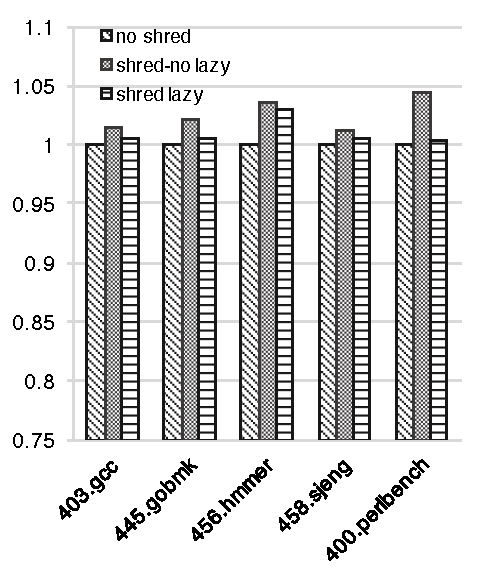
\includegraphics[scale=0.75]{shreds/figures/system_overhead}
%\caption{Five SPEC2000 benchmark programs tested when: (1) no shred is used, (2) shreds are used but without the lazy domain adjustment turned on in S-driver, and (3) shreds are used with the lazy domain adjustment. }
%\label{fig:sysoverhead}
%\end{center}
%\end{figure}



%end2end tests
In the end-to-end tests, we let each of the \numopensource open-source applications perform a self-contained task twice, with and without using shreds to protect their secret data (\eg Lighttpd fully handling an HTTP auth login and OpenSSL carrying out a complete RSA key verification). 
We instrumented the applications with timers. For each application, we manually drove it to perform the task, which fully exercises the added shreds. 
We measured both the time and space costs associated with using shreds in these tests. The absolute costs and the relative increases are shown in Table~\ref{tbl:e2e}.
On average, the per-task slow down among the applications is 4.67\% and the memory footprint increase is 7.26\%. 
The results show that shreds are practical for real applications of various sizes and functionalities. The overhead is hardly noticeable to the end users of the applications. 


\begin{table*}[t]
\begin{center}
\caption{End-to-end overhead observed while tested programs performing a complete task: the left-side part of the table shows the executing time and the right-side part shows the memory footprint.}
\label{tbl:e2e}
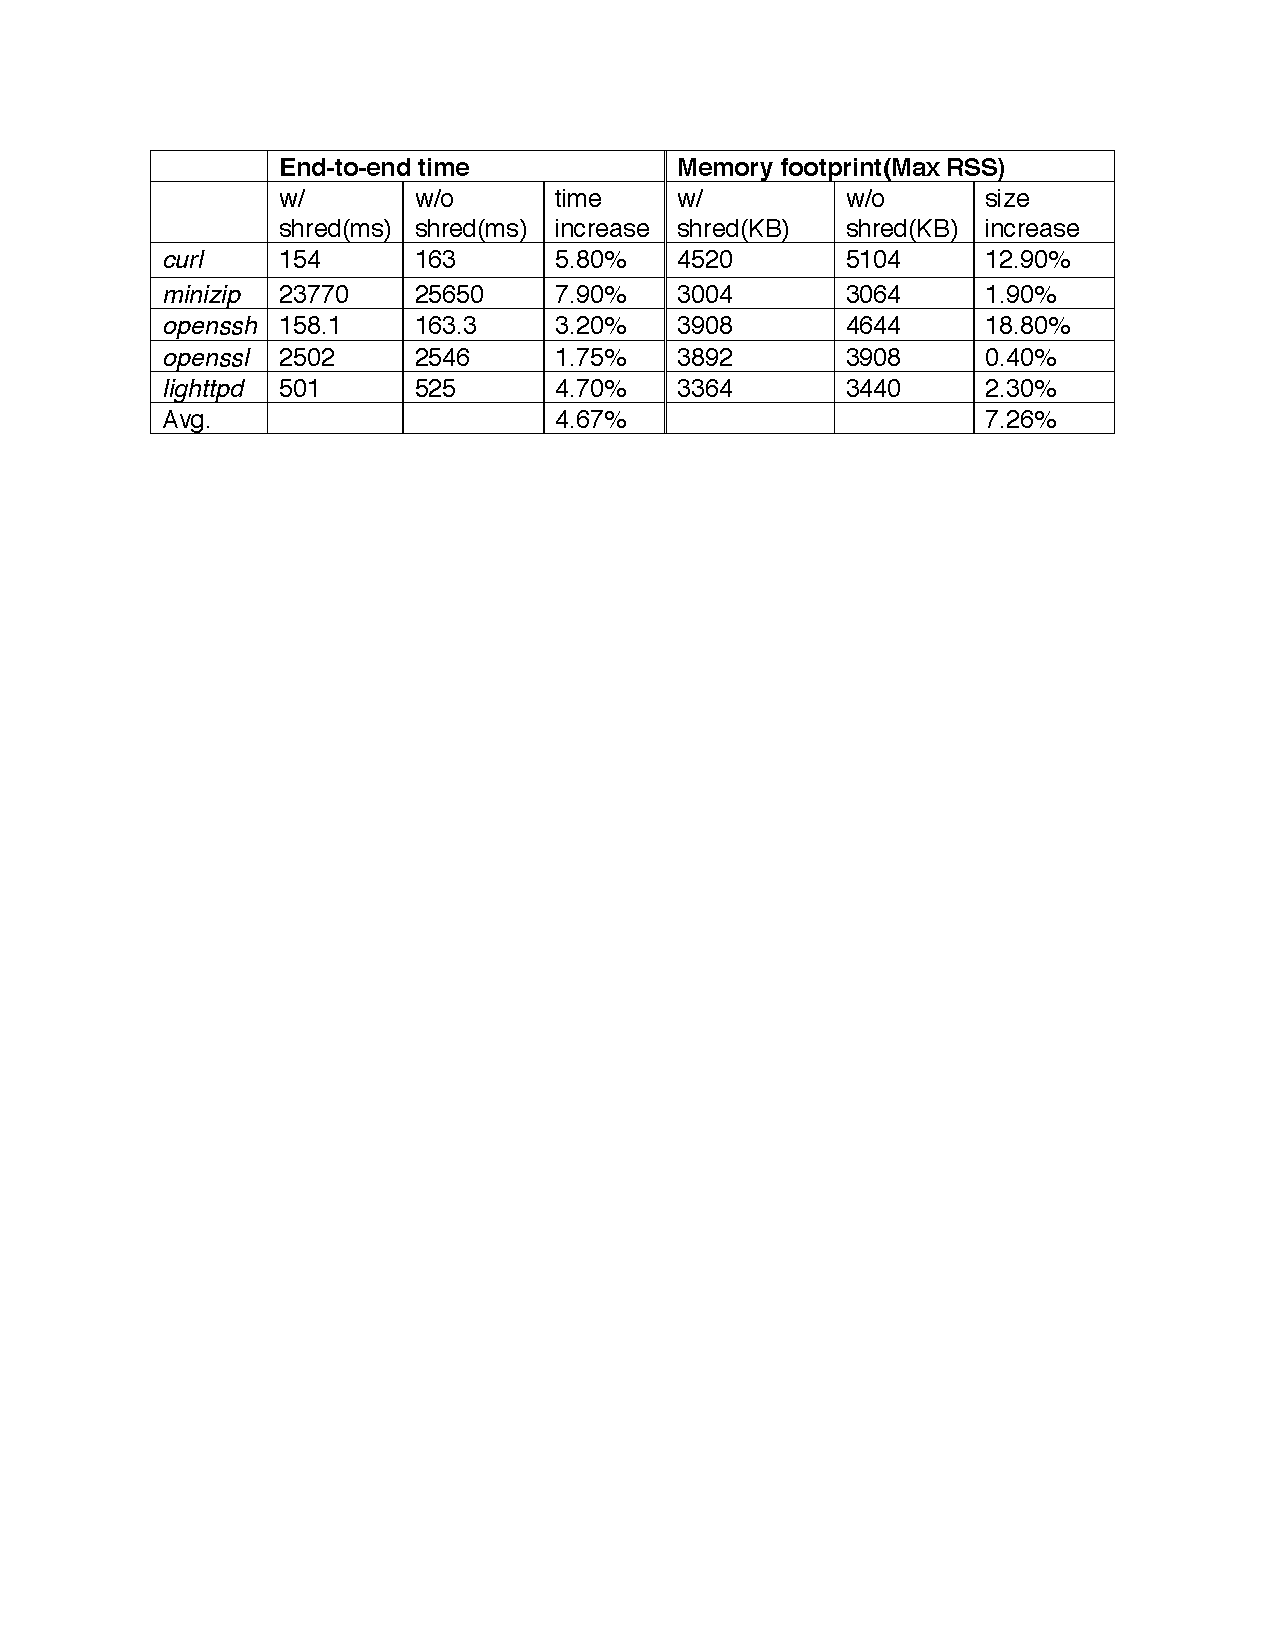
\includegraphics[scale=0.7]{shreds/figures/runtimeoverhead}
\end{center}
\end{table*}

\point{Security Coverage Test}
Finally, we tested the coverage of shred protection in the \numopensource modified applications. These tests not only check if the shred adoption is correct and complete in these applications, but also demonstrate the security benefits uniquely enabled by shreds in these applications. 
We conducted these tests using a simple memory scraper that scans each application's virtual memory in search for the known secrets. The tests simulate the most powerful in-process abuse where an adversary has full visibility into the user-space virtual memory of the application and can perform brute-force search of secrets. 
For each application, our memory scraper runs as an independent thread inside the application and verifies if any instance of the secret data can be found in memory via a value-based exhaustive search. We ran this test in two rounds, one on a vanilla version of the application and the other on the shred-enabled version. 

%exists outside of the s-pool (\ie an accident secret leak happened or the shred adoption was incomplete), and (2) if the s-pool is accessible by address (\ie the domain-based protection of s-pools is not correctly implemented). 

In the first round, where shreds are not used, the memory scraper found at lease one instance of the secret values in memory for all the applications, which means that these secrets are subject to in-process abuse. 
In the second round, where shreds are used, the memory scraper failed to detect any secrete matches in the applications' memory, which means that the secrets are well contained inside the s-pools and protected from  in-process abuse. 
The results show that, the applications have correctly adopted shreds for processing the secret data in memory and stored such data only in s-pools. Moreover, the tests show that, without significant design changes, applying the shred primitives in these real applications creates needed protection for the otherwise vulnerable passwords, crypto keys, and user credentials. 

